
\section{实验结果及分析}
\subsection{测试1}

使用SimplePLR类构建模型,进行已知断点位置的多段线性回归。对于给定的实例数据集,我们给出两种断点位置方案,分别为:

\[\begin{aligned}
    [min(x\_data), 0.039, 0.10, max(x\_data)]
    \\
    [min(x\_data), 0.050, 0.15, max(x\_data)]
    \end{aligned}\]

程序运行过后,所得到的结果分别为 \ref{image01} 和 \ref{image02}:

\begin{figure}[H]
    \centering
    \subfigure[]
    {
     \begin{minipage}{7cm}
      \centering
      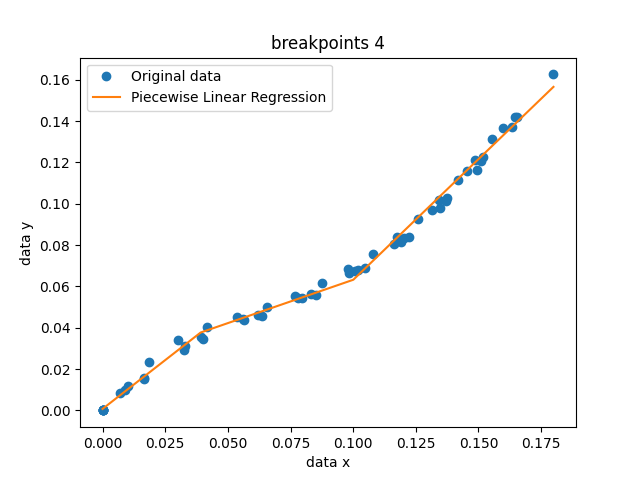
\includegraphics[scale=0.35]{./figure/chapter6/test1/image01.png}
      \label{image01}
     \end{minipage}
    }
       \subfigure[]
       {
        \begin{minipage}{7cm}
         \centering
         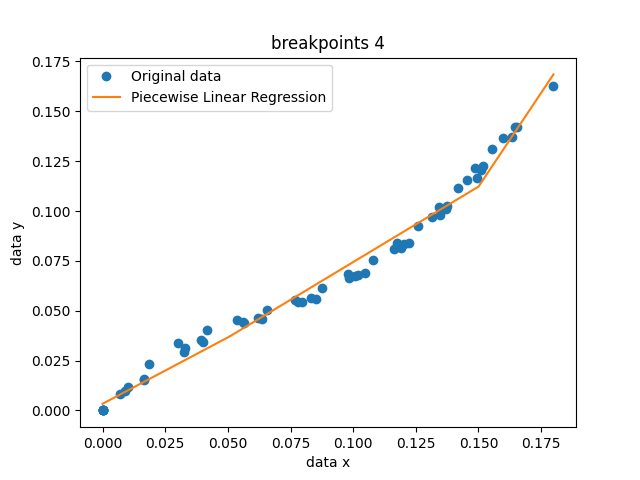
\includegraphics[scale=0.35]{./figure/chapter6/test1/image02.png}
         \label{image02}
        \end{minipage}
       }
   \caption{已知断点位置多段线性回归}
   \label{image0102}
   \end{figure}

同时,上述两种断点位置的分配对应的标准差和判定系数分别为:

\[\begin{aligned}
    SE(\beta_1)=[0.00096346,0.0388971,0.05737514,0.04040854]~
    R^2_1=0.99610201
    \\
    SE(\beta_2)=[0.00175845,0.05263311,0.07186705,0.16834045]~
    R^2_2=0.98563604
    \end{aligned}\]

通过观察上述曲线图像和相关系数可以知道,第一个断点位置分配更优。从这个测试中,我们也可以知道标准差和判定系数可以用于判断分段线性回归的效果。

\subsection{测试2}

使用 PLR 类构建模型,进行已知断点数目位置的多段线性回归。图 \ref{image03} 是分段数为5的运行结果,可以看到拟合曲线表现较不错。

\begin{figure}[H]
    \center{\includegraphics*[width = .8\textwidth]{./figure/chapter6/test2/image03.png}}
    \caption{PLR 模型构建全局最优的断点位置}
    \label{image03}      
\end{figure}

如此还可以继续改变分段的数目,并使用差分进化算法得到全局最佳的断点位置。这种思想在 \nameref{test3} 中得到了体现。


\subsection{测试3\label{test3}}

通过遍历多个分段数,每个分段数都输出拟合曲线的图像。同时生成判定系数随分段数增加而变化的曲线图。以下甄选出了一些典型分段数对应的拟合曲线,如图 \ref{test3} 所示。同时,还绘制了判定系数的变化曲线,如图 \ref{r_squares} 所示。

从图中可以看到,当分段数增加时,虽然标准差和判定系数都会变得更好,但是从图中直观来看,分段数增加到一定数目之后,拟合曲线就会出现毛刺(这一般是不被期望的),也就是说分段数过多会导致数据过拟合的情况,因此并不是分段数越多越优。

从判别系数随分段数变化曲线也可以看到,开始时,判别系数随分段数增加而显著增加;而当分段数增加到一定量后继续增加时,判别系数增加速度显著下降,并逐渐趋近$1$。以上测试结果对我们实际应用中的启示是,应该选择合适的分段数使得各种判定的数值足够优秀且避免数据过拟合的情况。

\begin{figure}[H]
    %\begin{tabular}{cc}   
    \begin{minipage}{0.48\linewidth}
      \centerline{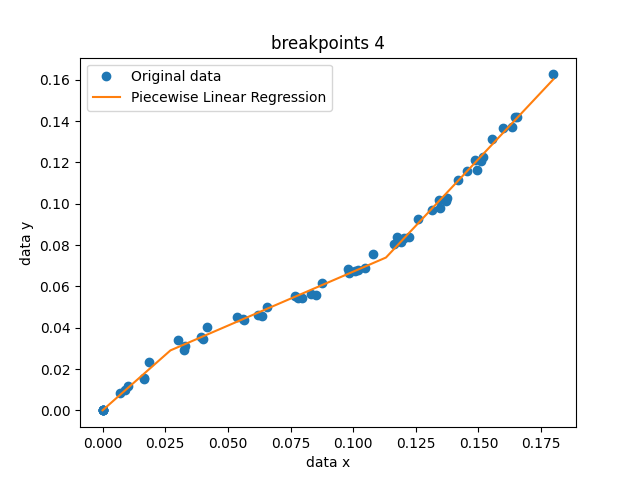
\includegraphics[width=8.0cm]{./figure/chapter6/test3/segment03.png}}
      \centerline{(a) segment 3}
    \end{minipage}
    \hfill
    \begin{minipage}{.48\linewidth}
      \centerline{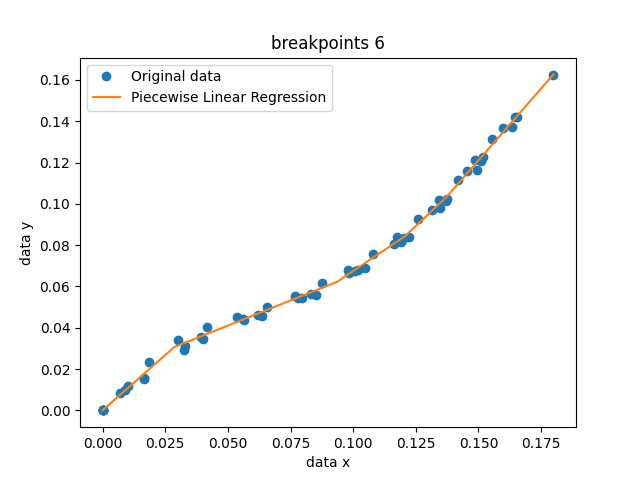
\includegraphics[width=8.0cm]{./figure/chapter6/test3/segment05.png}}
      \centerline{(b) segment 5}
    \end{minipage}
    \vfill
    \begin{minipage}{0.48\linewidth}
      \centerline{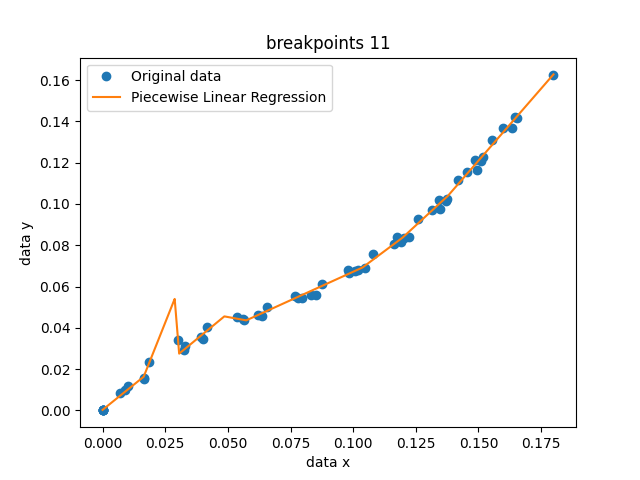
\includegraphics[width=8.0cm]{./figure/chapter6/test3/segment10.png}}
      \centerline{(c) segment 10}
    \end{minipage}
    \hfill
    \begin{minipage}{0.48\linewidth}
      \centerline{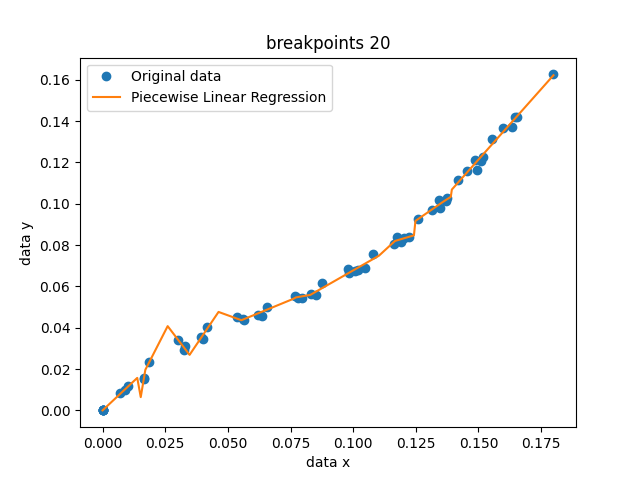
\includegraphics[width=8.0cm]{./figure/chapter6/test3/segment19.png}}
      \centerline{(d) segment 19}
    \end{minipage}
    %\end{tabular}
    \caption{各种不同分段数对应的线性拟合}
    \label{test3}
\end{figure}

\begin{figure}[H]
    \center{\includegraphics*[width = .6\textwidth]{./figure/chapter6/test3/r_squares.png}}
    \caption{判别系数随分段数增加的变化}
    \label{r_squares}      
\end{figure}

\subsection{测试4\label{test4}}

测试差分进化算法的收敛速度。这个测试对不同维数的数据,根据相同的评价函数,得到评价函数的最小值与迭代次数之间的关系如图 \ref{diffe} 所示。

\begin{figure}[H]
    \center{\includegraphics*[width = .7\textwidth]{./figure/chapter6/test4/de.png}}
    \caption{判别系数随分段数增加的变化}
    \label{diffe}      
\end{figure}

从图中可以看出,随着数据维数不断提高,差分进化算法收敛至全局最优点的迭代数不断增加。正如前文 \nameref{p2} 提到的,差分进化算法的收敛速度事实上随着维数的增加而呈指数型增加的趋势。所以,面对维数较大的数据集,比如Facebook 的经典评论数据集($54$维),该算法很可能开销难以容忍。

\subsection{测试5}

对于给定的实例数据集,通过 PLR 类建立模型,考察差分进化算法的收敛速度。这个测试与 \nameref{test4} 异曲同工,只是数据集更加具有普适性和一般性。测试的收敛速度如图 \ref{diffe_real} 所示。

从图中可以看出,该测试结果与 \nameref{test4} 显著不同,对于不同分段数,其最后收敛的值不同,原因是,对于一个真实数据集,不同分段数作用于数据集的效果是不同的。这也为我们找到全局最优分段数提供了思路,我们可以找到具有最小收敛$SS_{res}$值的分段数作为全局最优分段数。但是,这样的想法也是有问题,因为如果$segment = n$,则$SS_{res}$将等于$0$。

\begin{figure}[H]
    \center{\includegraphics*[width = .7\textwidth]{./figure/chapter6/test5/de_real.png}}
    \caption{判别系数随分段数增加的变化}
    \label{diffe_real}      
\end{figure}

回到图像本身,对于不同的分段数,算法收敛的速度是不一样的,一个显而易见的结论是,最终收敛值越小,所需的迭代次数越多。当然,这其中也有反例,比如segment7的收敛速度比segment6收敛速度快。因为本实验中采用$rand/1/bin$的策略,所以每次运行的结果也都是不同的。


\subsection{测试6}

这个测试中,观察分段线性回归模型对于非多项式函数的拟合情况。采用不同分段数对数据集进行拟合。结果如图 \ref{test6} 所示。其中源数据是从函数$y=cosx$进行偏置震荡得来的,如图 \ref{poly2} 所示;拟合曲线如图 \ref{poly1} 所示。

从图中可以看到,不同分段数对应的拟合曲线差别不大。也就是说,在分段数不大的情况下,拟合的曲线就已经可以反映数据集的大致分布。这给我们的启发是,在实际运用多段线性回归时,不一定需要选择较大的分段数或者全局最优分段数,在较小的分段数下,我们就可以得到曲线的大致分布,并且开销较小(差分进化算法开销随维数增加而指数型增加)。

\begin{figure}[H]
    \centering
    \subfigure[]
    {
     \begin{minipage}{7cm}
      \centering
      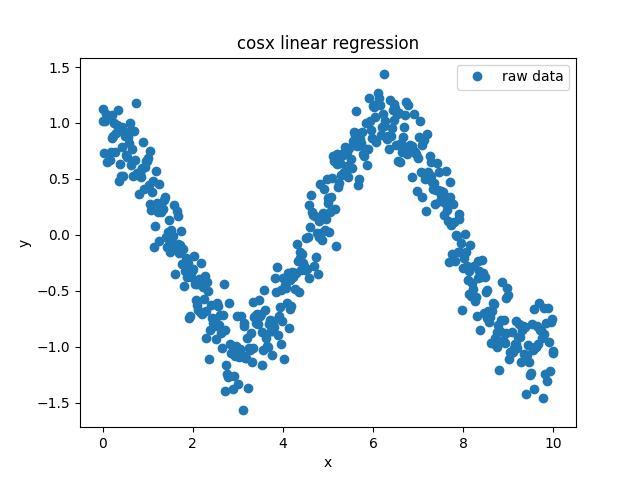
\includegraphics[scale=0.35]{./figure/chapter6/test6/poly2.png}
      \label{poly2}
     \end{minipage}
    }
       \subfigure[]
       {
        \begin{minipage}{7cm}
         \centering
         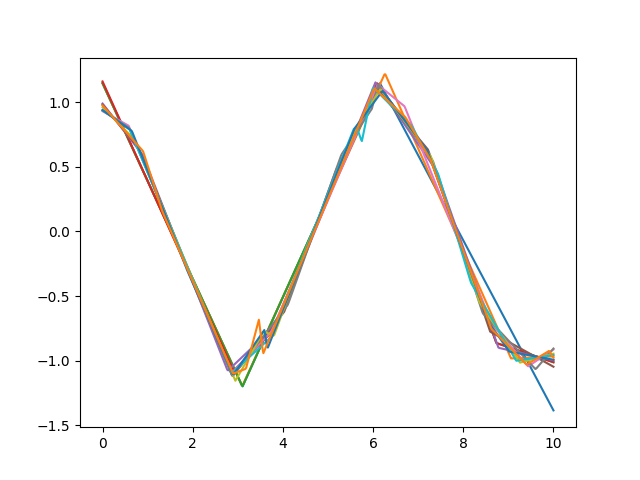
\includegraphics[scale=0.35]{./figure/chapter6/test6/poly1.png}
         \label{poly1}
        \end{minipage}
       }
   \caption{非多项式数据集拟合}
   \label{test6}
   \end{figure}

\subsection{应用结果}

分段线性回归的应用场景非常丰富,本次实验选取股票走势拟合进行简单的应用。首先,使用baostock第三方库调取的上证指数数据可视化后如图 \ref{app1} 所示。观察数据的大致走势,设置好一些列待检的分段数,使用 PLR 类建立模型并进行训练,每个分段数对应的分段函数如 \ref{app2} 图所示。

\begin{figure}[H]
    \center{\includegraphics*[width = 1\textwidth]{./figure/chapter6/app/app1.jpg}}
    \caption{真实数据:上证指数}
    \label{app1}      
\end{figure}

从图上可以看出,拟合的大致效果还是不错的,基本上可以反映出上证指数的走势情况。

\begin{figure}[H]
    \center{\includegraphics*[width = 1\textwidth]{./figure/chapter6/app/app2.jpg}}
    \caption{实际应用:股票拟合}
    \label{app2}      
\end{figure}


综上所示,本次实验的目的已经达到。面对一个数据集,如果在观察到可以使用多段线性回归来对模型进行拟合的情况下,我们可以选用本次使用中使用的方法。首先是对问题进行建模,通过源数据生成回归矩阵,将多段线性回归问题转换成单一线性回归问题,再使用差分进化算法来对残差平方和进行全局优化得到全局最优的$\beta$参数,即断点的位置。